\documentclass{article}
\usepackage[utf8]{inputenc}

\title{Data Mining - Blatt 04}
\author{Manuel, Marius}
\date{\today}

\usepackage{natbib}
\usepackage{graphicx}
\usepackage{subfigure}

\usepackage{listings}
\usepackage{color}

%from https://stackoverflow.com/questions/3175105/writing-code-in-latex-document
\definecolor{dkgreen}{rgb}{0,0.6,0}
\definecolor{gray}{rgb}{0.5,0.5,0.5}
\definecolor{mauve}{rgb}{0.58,0,0.82}

\lstset{frame=tb,
	language=Java,
	aboveskip=3mm,
	belowskip=3mm,
	showstringspaces=false,
	columns=flexible,
	basicstyle={\small\ttfamily},
	numbers=none,
	numberstyle=\tiny\color{gray},
	keywordstyle=\color{blue},
	commentstyle=\color{dkgreen},
	stringstyle=\color{mauve},
	breaklines=true,
	breakatwhitespace=true,
	tabsize=3
}


\begin{document}

\maketitle

\section{Abgabe Übung 4}
Im Folgenden sind die Plots der einzelnen Konfigurationen der Algorithmen. Leider war es uns nicht möglich das Dataset S2 mit den Algorithmen durchlaufen zu lassen. Wir haben es für mehrere Stunden auf dem Computer laufen lassen, jedoch ohne Erfolg. Auch die Plots wurden trotz vielem Probieren und Ändern der Plot-Funktion nicht wirklich besser.
agnes diana

\begin{figure}[ht!]
\caption{Detaset Seeds}
\centering
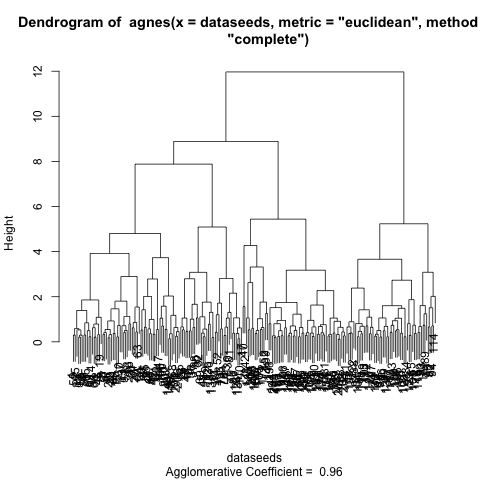
\includegraphics[width=1\textwidth]{plots/ang1dataseeds.png}
\end{figure}

\begin{figure}[ht!]
\caption{Detaset Seeds}
\centering
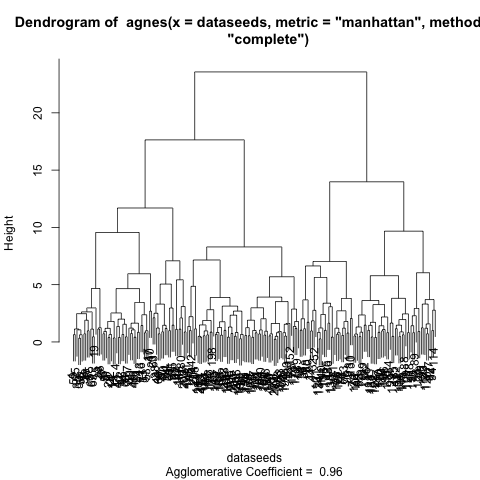
\includegraphics[width=1\textwidth]{plots/ang2dataseeds.png}
\end{figure}

\begin{figure}[ht!]
\caption{Detaset Seeds}
\centering
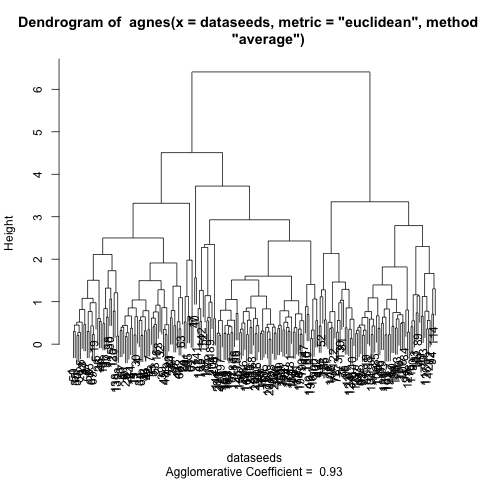
\includegraphics[width=1\textwidth]{plots/ang3dataseeds.png}
\end{figure}

\begin{figure}[ht!]
\caption{Detaset Seeds}
\centering
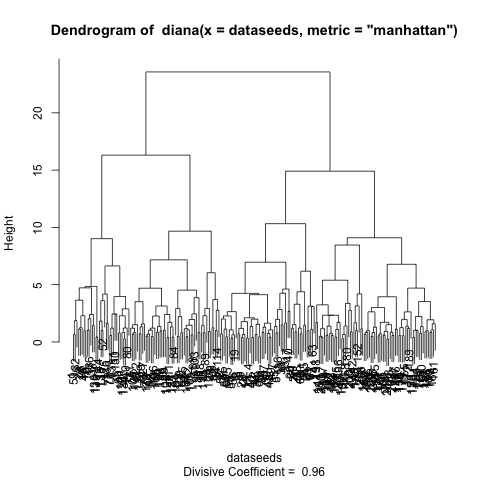
\includegraphics[width=1\textwidth]{plots/dv1dataseeds.png}
\end{figure}

\begin{figure}[ht!]
\caption{Detaset Seeds}
\centering
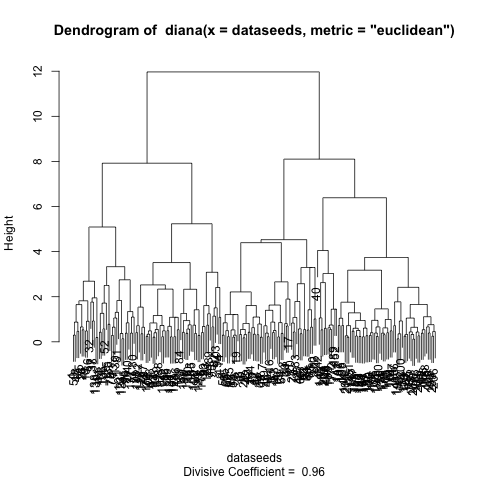
\includegraphics[width=1\textwidth]{plots/dv2dataseeds.png}
\end{figure}

\begin{figure}[ht!]
\caption{Detaset Dim032}
\centering
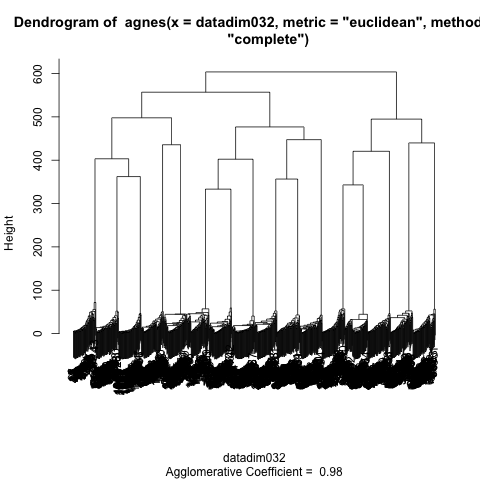
\includegraphics[width=1\textwidth]{plots/ang1dim032.png}
\end{figure}

\begin{figure}[ht!]
\caption{Detaset Dim032}
\centering
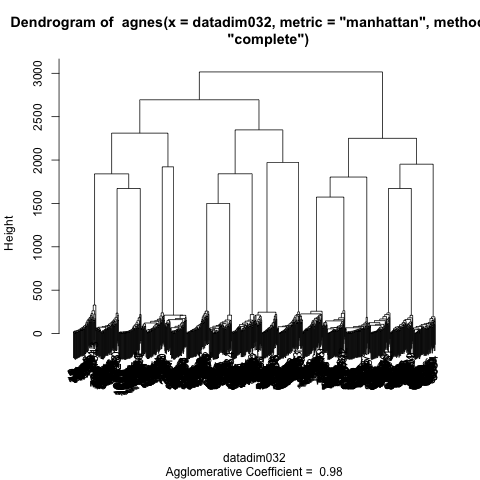
\includegraphics[width=1\textwidth]{plots/ang2dim032.png}
\end{figure}

\begin{figure}[ht!]
\caption{Detaset Dim032}
\centering
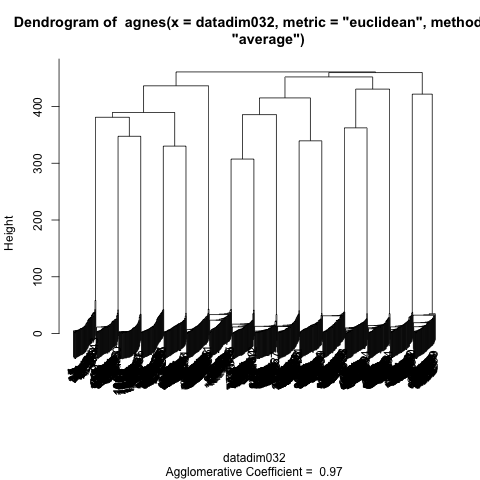
\includegraphics[width=1\textwidth]{plots/ang3dim032.png}
\end{figure}

\begin{figure}[ht!]
\caption{Detaset Dim032}
\centering
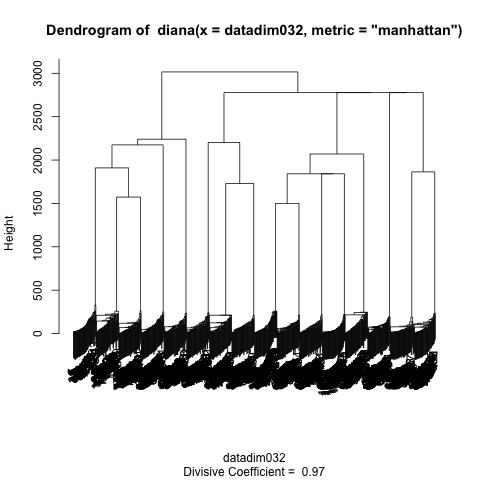
\includegraphics[width=1\textwidth]{plots/dv1dim032.png}
\end{figure}

\begin{figure}[ht!]
\caption{Detaset Dim032}
\centering
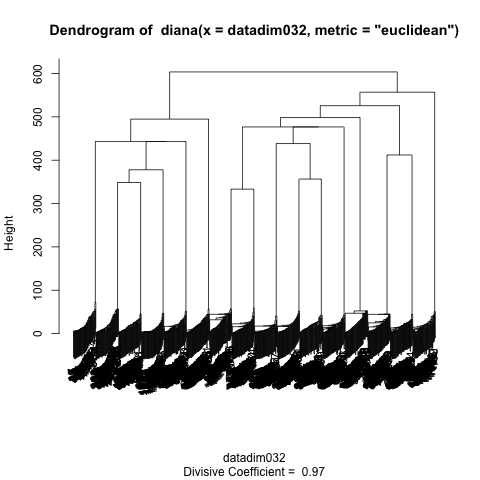
\includegraphics[width=1\textwidth]{plots/dv2dim032.png}
\end{figure}

Da die Plots nicht wirklich gut sind konnten wir daraus nicht sehr viel über die Datensätze lernen. Jedoch beschreiben wir im folgenden die Hierarchische Clusteranalyse.

\subsection{Hierarchische Clusteranalyse}
Bei der hierarchischen Clusteranalyse wird mittels distanzbasierten Verfahren eine Clusteranalyse durchgeführt. Ein Cluster besteht dabei aus Objekten, welche zueinander eine höhere Ähnlichkeit haben als zu Objekten eines anderen Clusters. \\
Die Verfahren der hierarchischen Clusteranalyse können durch die verwendeten Distanz- bzw. Proximitätsmaßen aufgeteilt werden. Ebenso spielt die Berechnungsvorschrift eine Rolle. Anhand derere können zwei wichtige Typen von Verfahren benannt werden. \\
\\
"Top-down-Verfahren": Hierbei werden zuerst alle Objekte einem Cluster zugeordnet und das so gebildete Cluster in kleinere Cluster aufgeteilt. Bis nur noch ein Objekt in einem Cluster ist.
\\
"Bottom-up-Verfahren": Hier wird zuerst jedem Objekt ein Cluster zugeordnet und dann nach und nach die bereits gebildeten Cluster solange zusammengefasst bis alle Objekte zu einem Cluster gehören. 
\\
Allgemein gilt, dass gebildete Cluster nicht mehr verändert werden können. Nur die Struktur der Cluster wird somit entweder verfeinert oder vergröbert. \footnote{https://de.wikipedia.org/wiki/Hierarchische\_Clusteranalyse}

\end{document}
